\documentclass[conference]{IEEEtran}
% Sem fomento informado: sem \thanks, sem \IEEEoverridecommandlockouts. Se houver fomento,
% acrescentar \IEEEoverridecommandlockouts aqui e \thanks{...} no título.

\usepackage{cite}
\usepackage{amsmath,amssymb,amsfonts}
\usepackage{graphicx}
\usepackage{textcomp}
\usepackage{xcolor}
\usepackage{url} % DOIs das referências: quebra em / e . sem inserir hífen
\graphicspath{{img/}{figures/}}

% Regras: CLAUDE.md. Sem travessão no fonte, no PDF e nas referências. Todo número de
% resultado sai de analysis/extract_results.py (analysis/out/summary.json, tables/results.tex).
% Autores: placeholders até o autor informar (TAREFAS.md).

\begin{document}
\bstctlcite{BSTcontrol}

\title{From Rotordynamic Model to Real-Time Firmware: Embedded Linear Quadratic Gaussian Control of an Active Magnetic Bearing Test Bench}

% Placeholders sem colchete: depois de \\ um [ vira argumento opcional de espaçamento.
\author{\IEEEauthorblockN{TODO 1st author}
\IEEEauthorblockA{\textit{TODO department} \\
\textit{TODO organization}\\
TODO city, country \\
TODO e-mail or ORCID}
\and
\IEEEauthorblockN{TODO 2nd author}
\IEEEauthorblockA{\textit{TODO department} \\
\textit{TODO organization}\\
TODO city, country \\
TODO e-mail or ORCID}
}

\maketitle

\begin{abstract}
Active magnetic bearings are open-loop unstable and need a stabilizing controller that meets tight timing limits on embedded hardware. This paper documents a complete path from a finite element rotordynamic model to a linear quadratic Gaussian controller that runs at 10 kHz on a dual-core TMS320F28379D microcontroller, and validates it on a low-cost vertical rotor test bench spun by an air jet. The design pipeline truncates the rotor model to two lateral mode pairs, expresses the state at the sensor location, adds input disturbance states that act as integral action, and computes the regulator and current estimator gains in discrete time. The firmware samples the proximity probes at 40 kHz in step with the pulse width modulation, removes an interference tone with an adaptive notch filter, and drives four coils with a differential bias scheme through H-bridges without current sensing. In three recordings of 300 s at increasing blower levels, the loop kept its 10 kHz rate without a single error, the embedded speed estimator agreed with handheld tachometer peaks within 2 percent, and the RMS position error grew from about 147 to 205 micrometers, mostly at the rotation frequency. The Y axis carried a constant control current of about 52 milliamperes and saturated in up to 10 percent of the control cycles. A comparison with the design model traces these departures to unmodeled synchronous excitation and axis asymmetry, which define the next design iteration.
\end{abstract}

\begin{IEEEkeywords}
active magnetic bearings, embedded control, flywheel energy storage, linear quadratic Gaussian control, real-time systems, rotordynamics
\end{IEEEkeywords}

\section{Introduction}\label{sec:intro}

Flywheel energy storage systems (FESS) offer high power density and long cycle life, and their efficiency depends on keeping friction and drag losses low at high speed~\cite{choudhury2021flywheel}. Active magnetic bearings (AMB) remove contact friction and allow operation in vacuum, which is why they appear in many FESS designs~\cite{schweitzer2009magnetic,du2025review}. An attraction-type AMB has negative position stiffness: the force grows as the rotor approaches the electromagnet, so the rotor is unstable without feedback and the controller must act on every sample, within a fixed period, for as long as the machine runs~\cite{schweitzer2009magnetic}.

Decentralized proportional-integral-derivative (PID) control is the industrial default, while model-based multivariable controllers handle rotor flexibility, gyroscopic coupling and non-collocated sensors more directly~\cite{wu2025review,du2025review}. The linear quadratic Gaussian (LQG) controller combines a linear quadratic regulator (LQR) with a Kalman filter~\cite{kalman1960new}, but it has no guaranteed stability margins~\cite{doyle1978guaranteed}, so its design must be checked against model uncertainty before it reaches hardware. Experimental work has moved such controllers from simulation to prototypes. Castellanos Molina \emph{et al.} implemented offset-free model predictive control on a cone-shaped AMB test rig~\cite{castellanos2021offset}. Zhao \emph{et al.} combined linear state-feedback decoupling with current compensation and validated it on a 100 kW maglev flywheel prototype whose controller board uses a TMS320F28377D, a device of the same family used here, with current-mode power amplifiers~\cite{zhao2026constraint}. Reports of this kind seldom describe the chain between the rotordynamic model and the deployed code: which state the firmware keeps, how the model is discretized and stored, how sampling is synchronized with switching, and what the embedded loop records about itself. Real-time hardware constraints also shape what can be identified and verified on a running AMB~\cite{wang2026identification}.

This paper documents that chain for a vertical rotor test bench that precedes a full-scale FESS. The bench is deliberately low cost: H-bridge drivers without current sensing, one proximity probe per axis, and an air jet as the drive. Its contributions are:
\begin{itemize}
\item a reproducible model-to-firmware pipeline, from an open-source finite element (FE) rotor model~\cite{timbo2020ross} to a ten-state discrete LQG controller with integral action, a robustness grid, and float32 export;
\item a real-time implementation on a dual-core microcontroller, with acquisition synchronized to the pulse width modulation (PWM), an adaptive notch filter, a 10 kHz control interrupt, differential bias actuation, safety interlocks and firmware window statistics;
\item experimental results at three rotation levels up to about 3500 rpm, compared with the design predictions and analyzed with explicit account of what the telemetry can and cannot show.
\end{itemize}
Section~\ref{sec:bench} describes the bench, Section~\ref{sec:pipeline} the design pipeline, Section~\ref{sec:implementation} the firmware, Section~\ref{sec:results} the results, Section~\ref{sec:discussion} compares the model with the bench, and Section~\ref{sec:limitations} lists the limitations.

\section{Test Bench}\label{sec:bench}

\begin{figure*}[tbp]
\centering
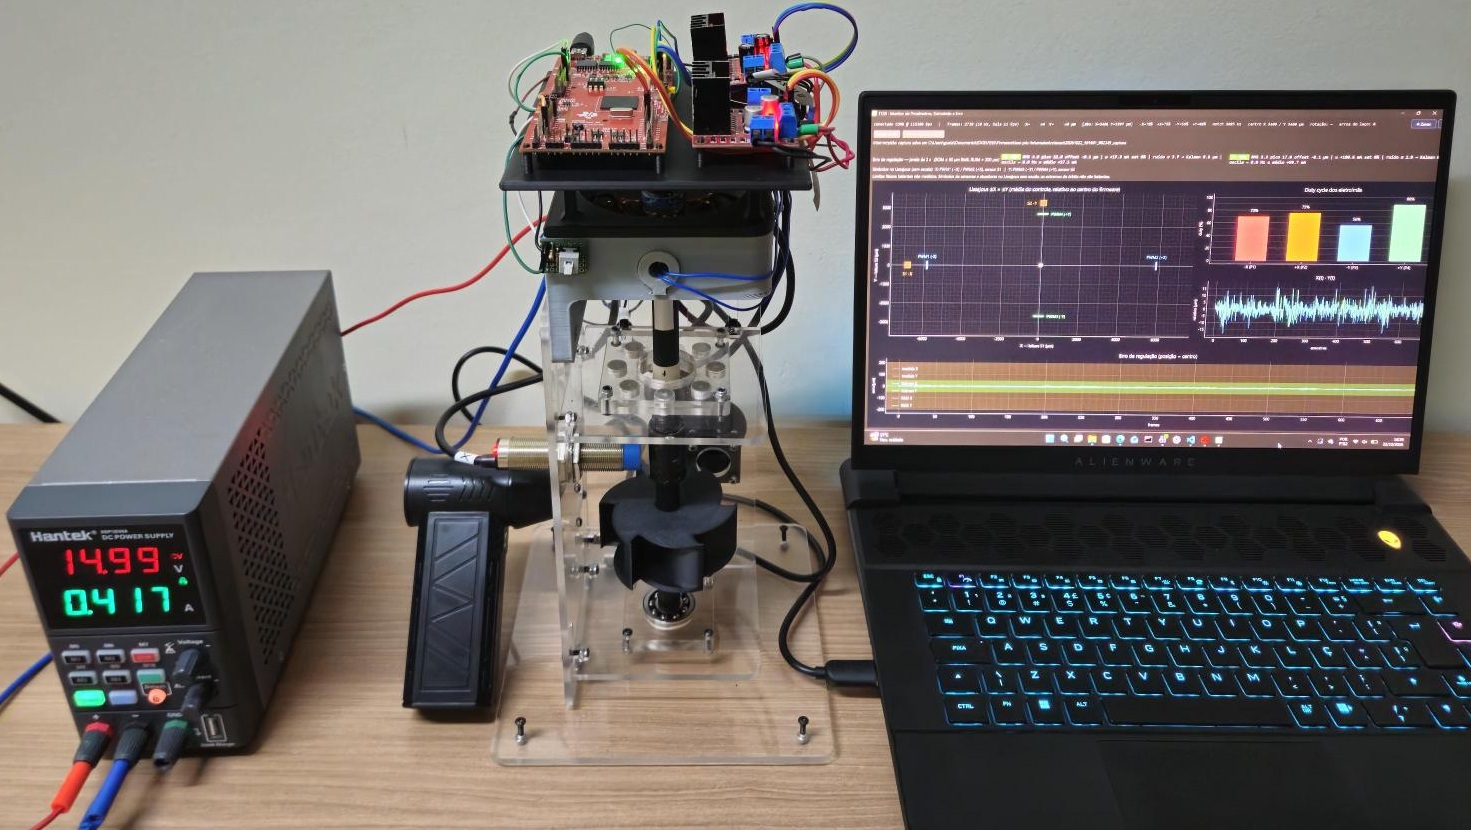
\includegraphics[height=1.75in]{bench_setup.jpg}\hfill
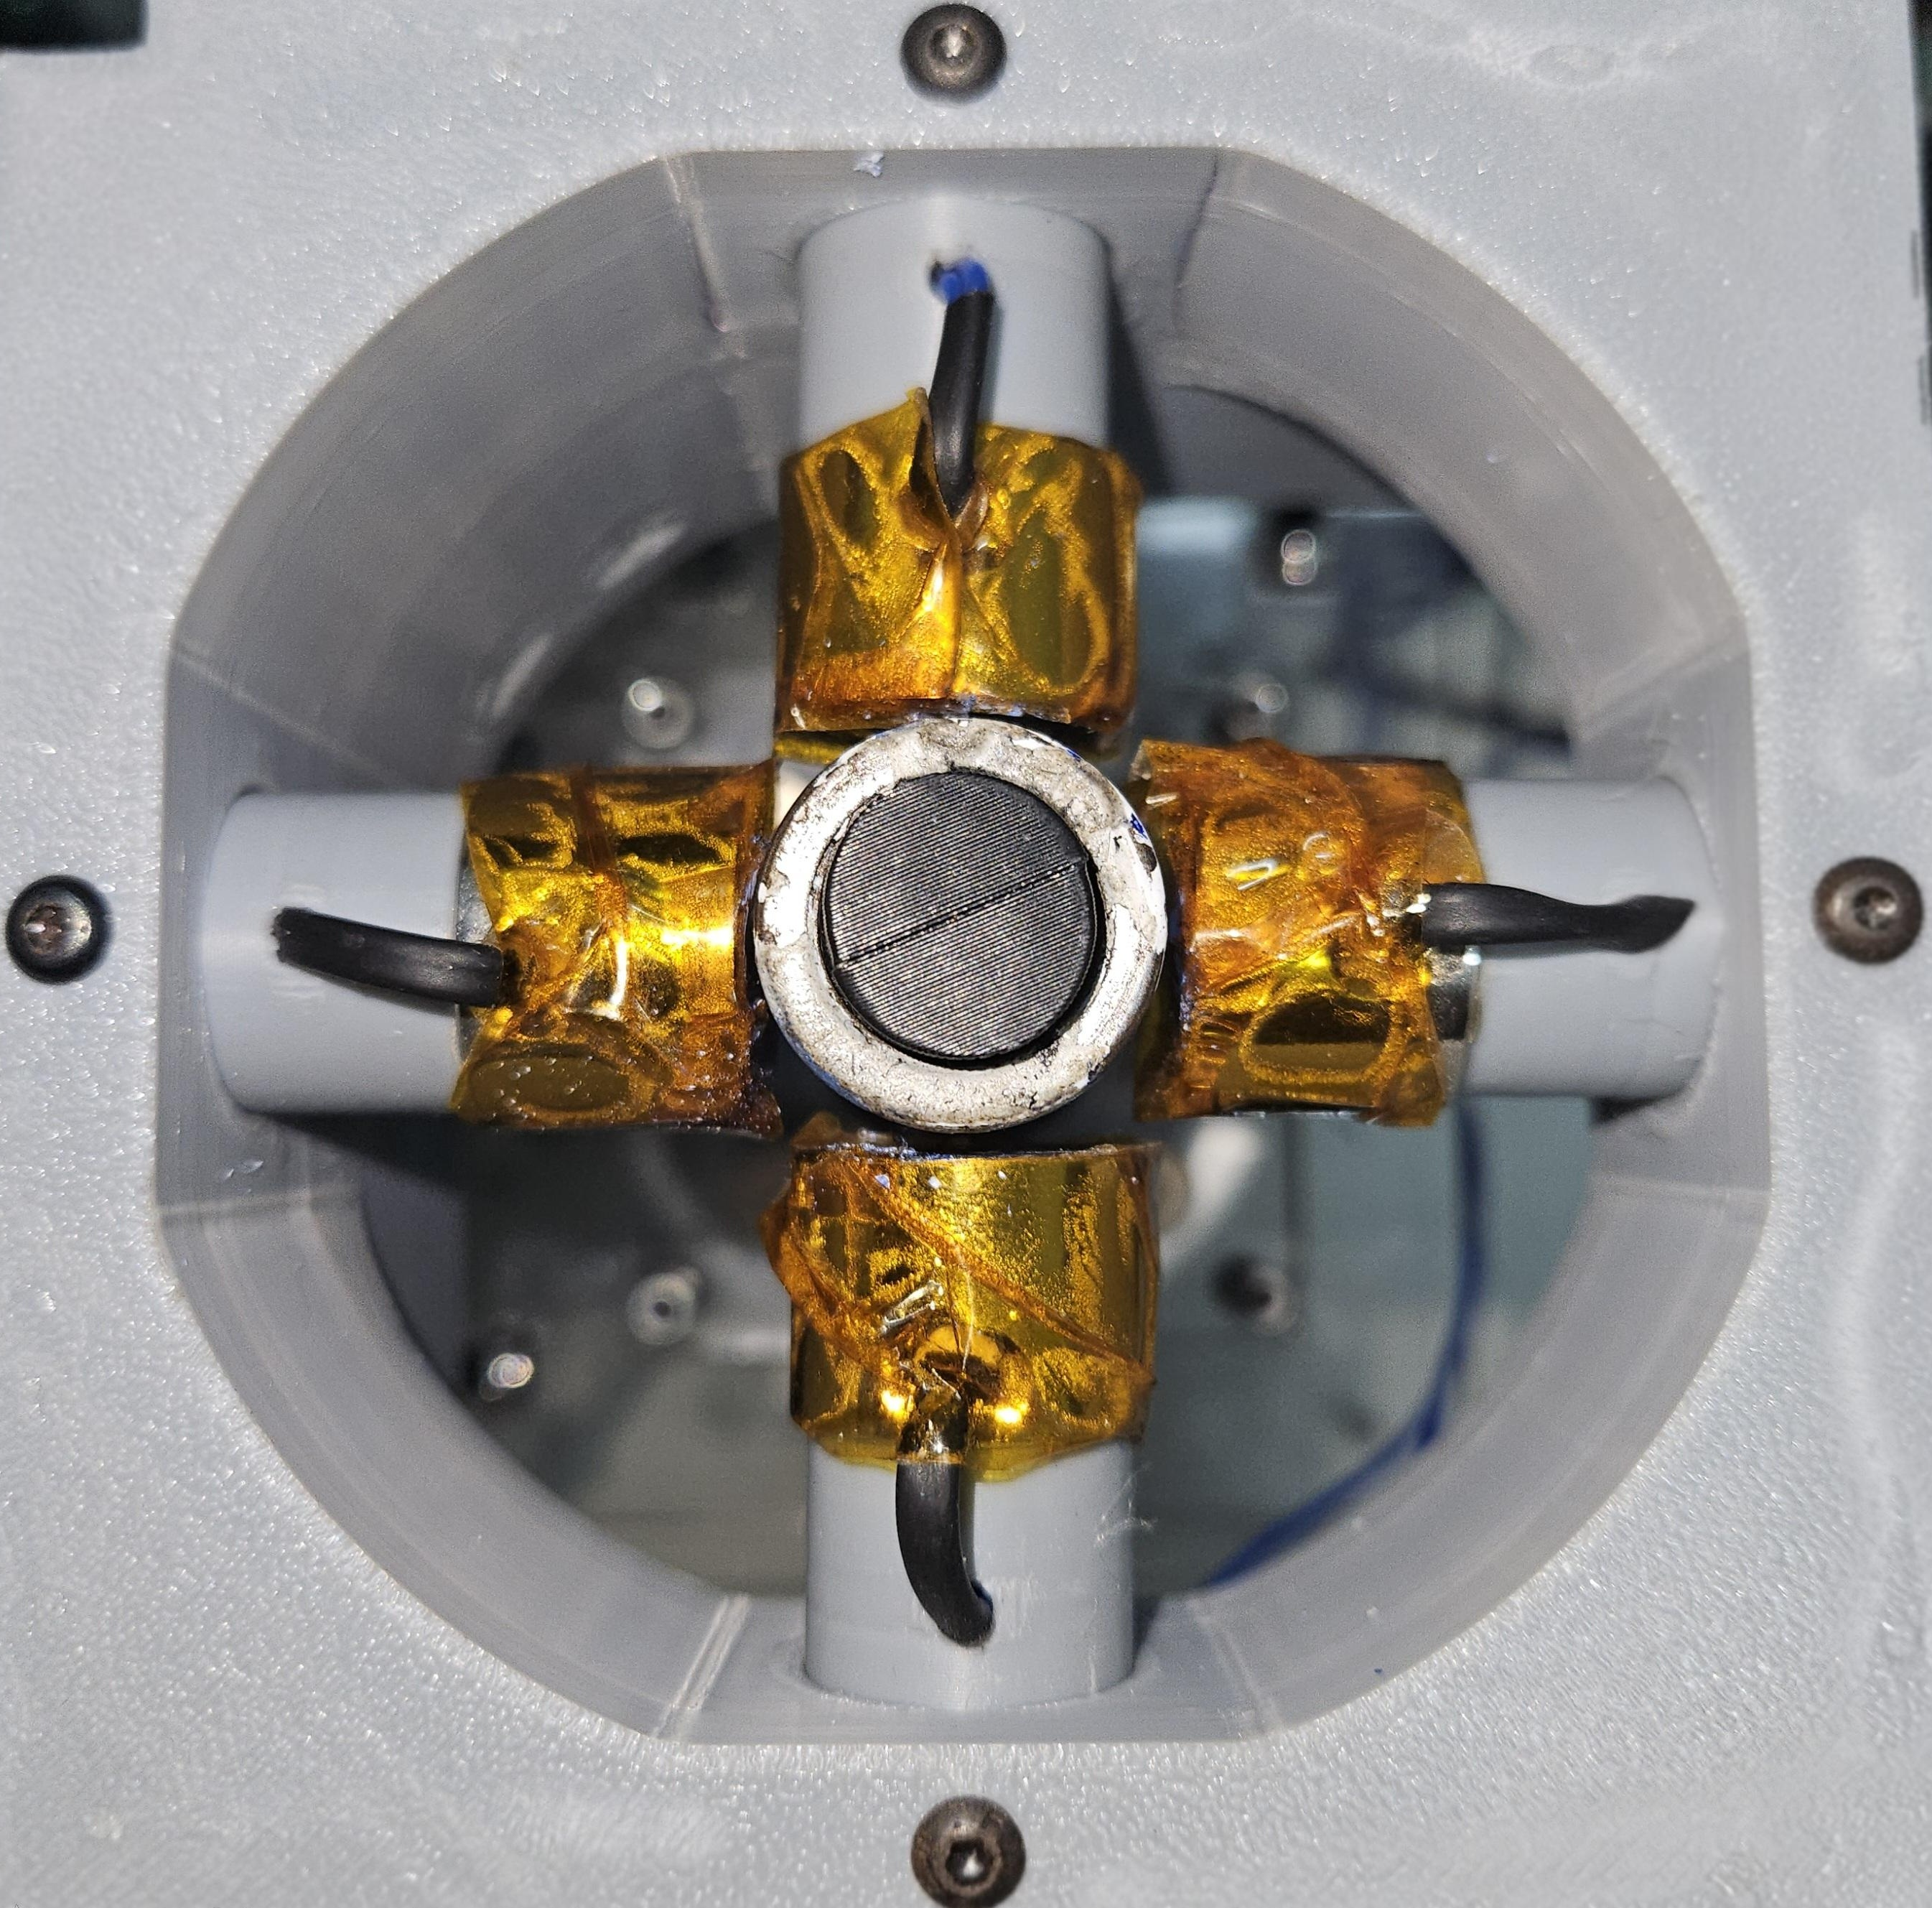
\includegraphics[height=1.75in]{mancal_magnetico_ativo.jpg}\hfill
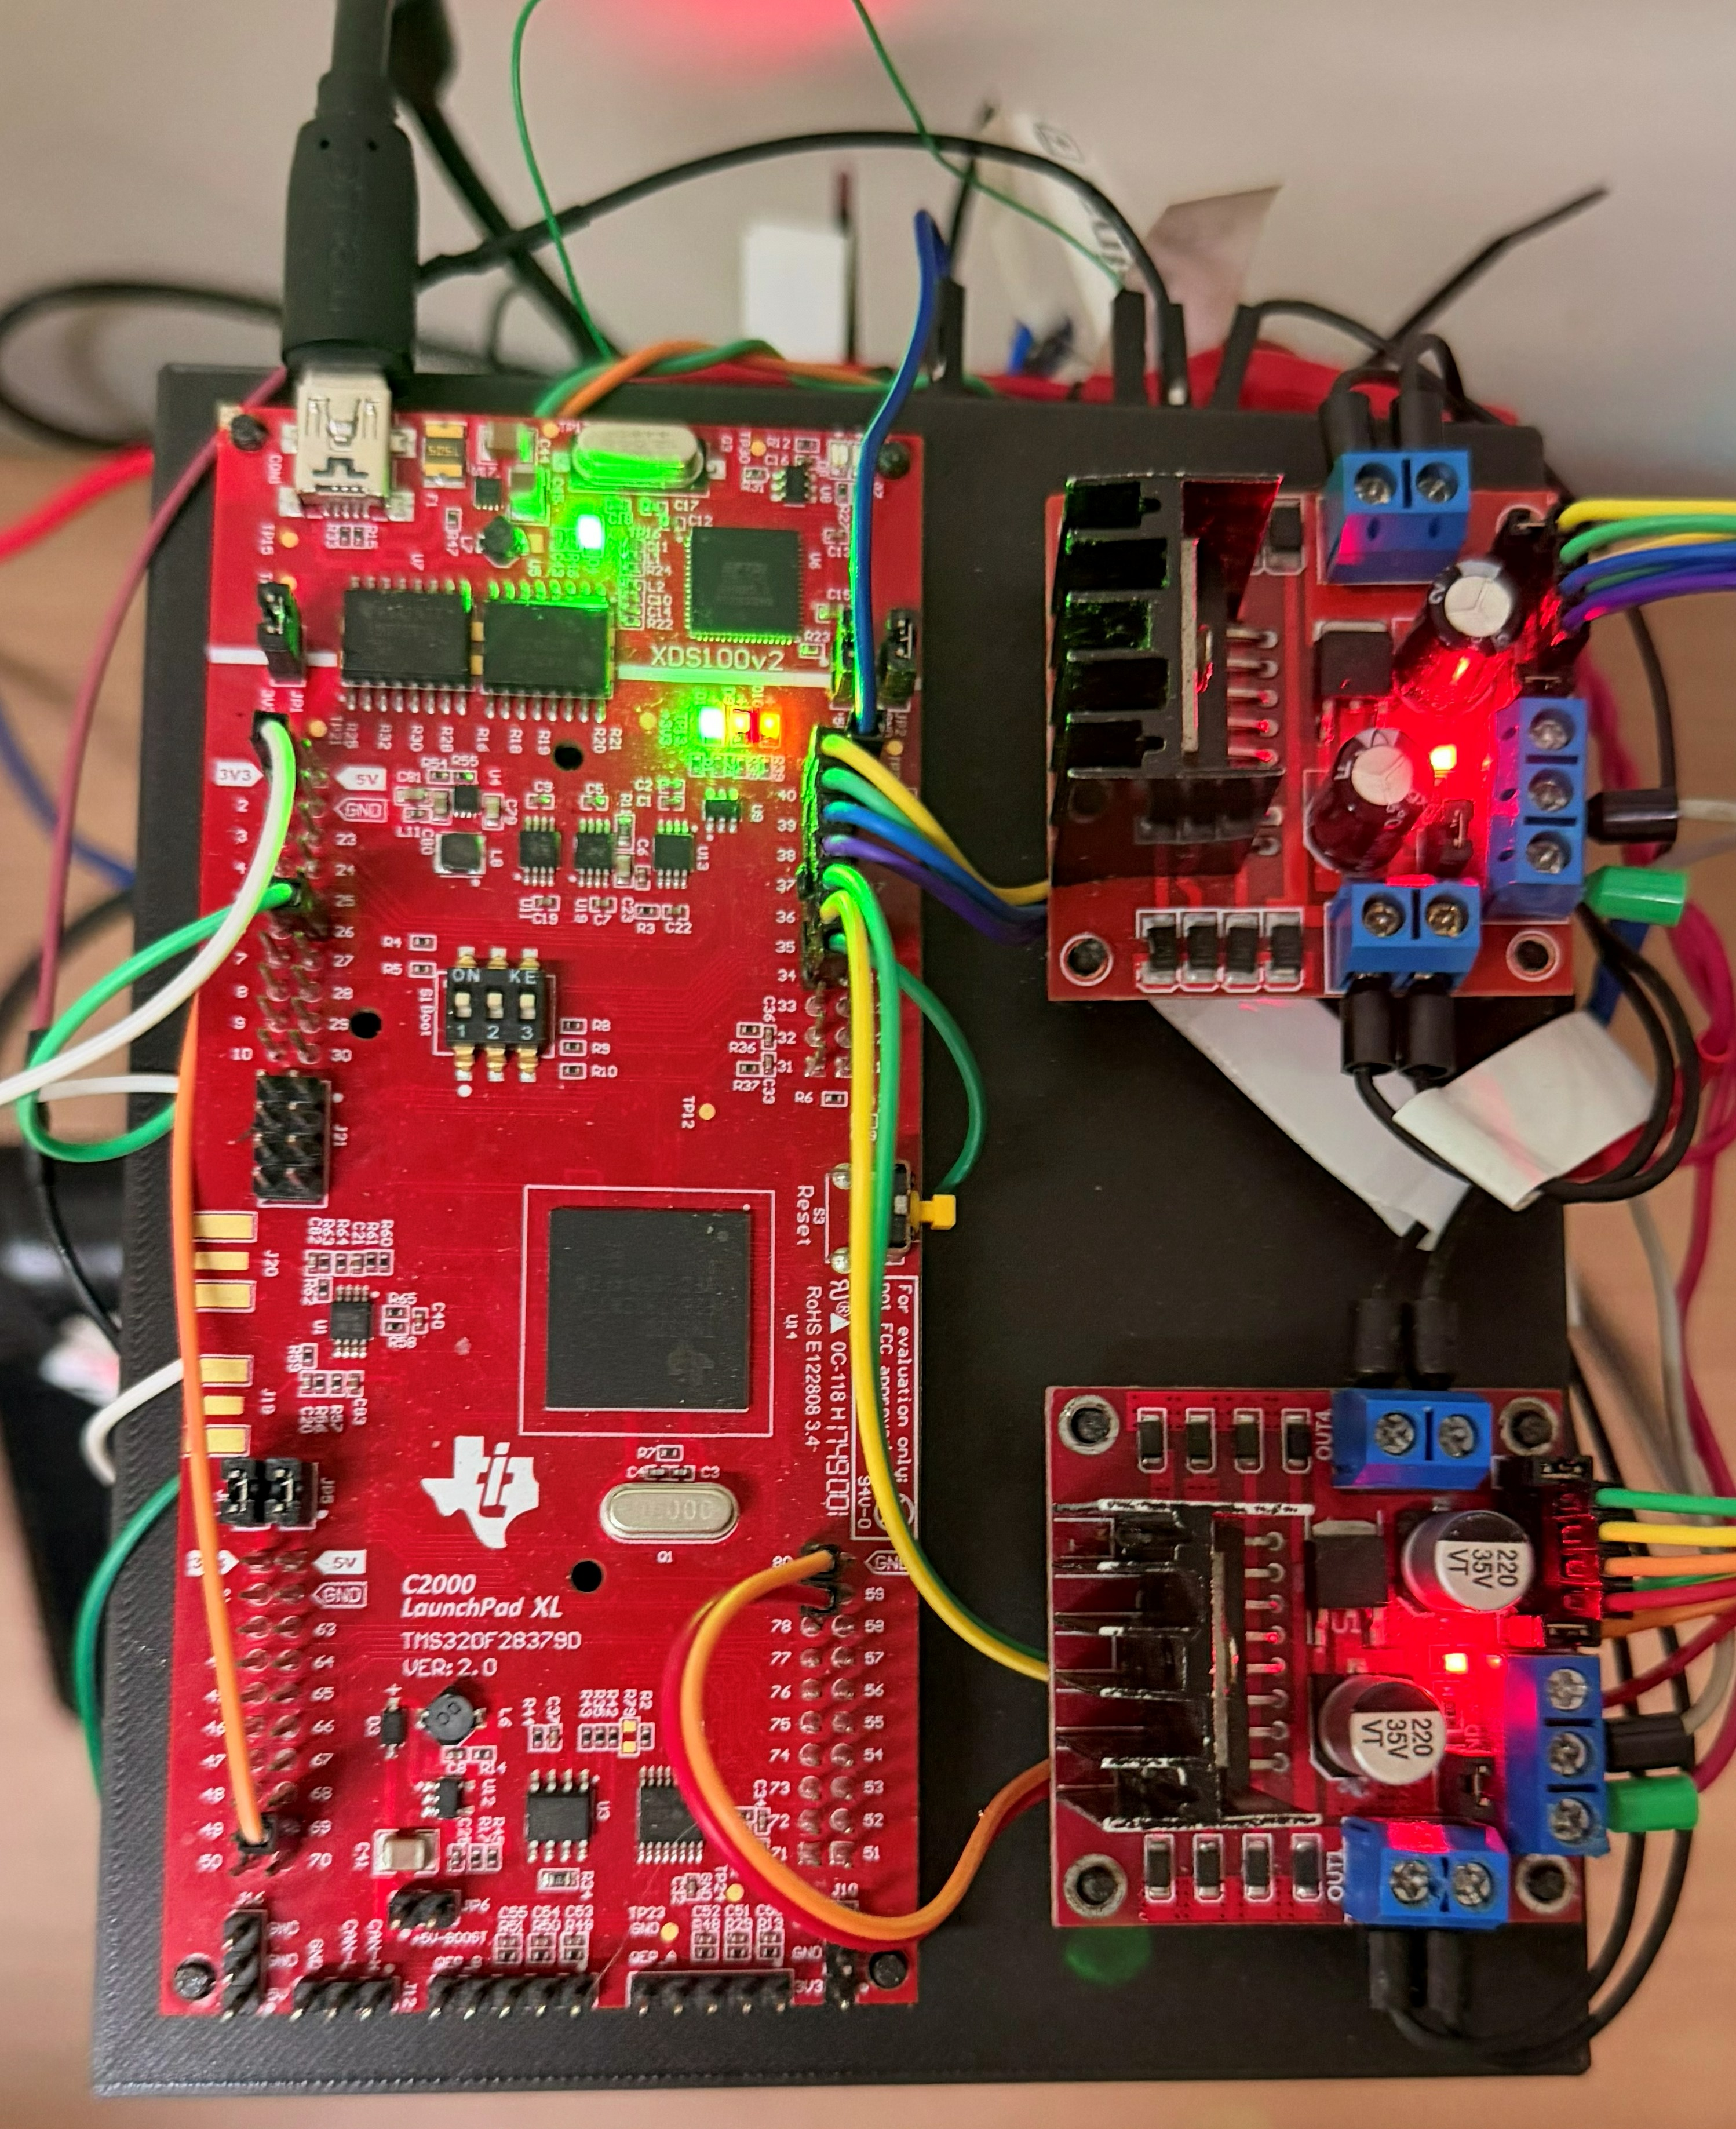
\includegraphics[height=1.75in]{launchf28379d_l298n.jpg}
\caption{Test bench. (a) Overview: 15 V supply, blower, vertical rotor, controller and monitoring computer. (b) Top view of the active magnetic bearing, with four electromagnets around the rotor target. (c) LaunchPad with the TMS320F28379D and two L298N dual H-bridge boards.}
\label{fig:bench}
\end{figure*}

The rotor (Fig.~\ref{fig:bench}) stands vertically on a 13 mm polylactic acid (PLA) shaft that carries concentrated masses: two target rings, the magnet of a permanent magnetic bearing (PMB), and an impeller. From top to bottom, the shaft passes through the AMB, the PMB, the proximity probes and the impeller, and rests on a rolling-element bearing that acts as a pivot. The PMB provides passive radial stiffness; the AMB, with four electromagnets in two opposing pairs, controls the two radial directions X and Y. The weight of the rotor rests on the pivot, so the AMB only centers the rotor and carries no static weight. A blower aimed at the impeller spins the rotor, and its three settings are the test conditions of Section~\ref{sec:results}.

One proximity probe per axis faces the lower target ring. The 12-bit analog-to-digital converter (ADC) of the microcontroller reads each probe, and a fourth-order polynomial per axis maps counts to distance over 1 to 6 mm, with maximum fitting residuals of 9.4 $\mu$m (X) and 16.7 $\mu$m (Y).

The controller is a LaunchPad board with a TMS320F28379D, which has two C28x cores at 200 MHz with single-precision floating-point units (FPU)~\cite{ti2024f2837xd}. The first core runs the control loop; the second only reads shared memory for supervision. Two L298N boards, supplied at 15 V, drive the four coils of 48 $\Omega$ each. There is no current sensor, so the commanded current is converted into a duty cycle under a steady-state assumption (Section~\ref{sec:actuation}).

A force test on one electromagnet was fitted to $F = k(i - i_d)^2/(g + g_\text{off})^2$ and linearized for a coil pair at the bias current $i_0 = 140$ mA and the nominal gap of 1.45 mm per side, which gives
\begin{equation}
f = k_i\, i + k_s\, x, \quad k_i = 5.37~\text{N/A}, \quad k_s = 403.3~\text{N/m}, \label{eq:force}
\end{equation}
where $f$ is the net force of the pair, $i$ the control current, and $x$ the rotor displacement at the bearing. The term $k_s x$ pushes the rotor further in the direction of its displacement, so it acts as a negative stiffness.

\section{Model-to-Firmware Pipeline}\label{sec:pipeline}

\subsection{Rotor Model}

The rotor is modeled in the Rotordynamic Open Source Software (ROSS)~\cite{timbo2020ross} with shaft elements that include shear deformation, rotary inertia and gyroscopic effects~\cite{friswell2010dynamics}, disk elements for the concentrated masses, and bearing elements for the pivot, the PMB and aerodynamic damping. Without the AMB, the lateral degrees of freedom $q$ obey
\begin{equation}
M\ddot{q} + (C + \Omega G)\dot{q} + K q = B_f\, f, \label{eq:fe}
\end{equation}
where $M$, $C$, $G$ and $K$ are the mass, damping, gyroscopic and stiffness matrices, $\Omega$ is the rotation speed, and $B_f$ applies the bearing force at the AMB node. Substituting \eqref{eq:force} adds $-k_s$ to the stiffness at that node and makes $k_i\,i$ the input. At design time the PMB had not been characterized: its stiffness was set to $10^3$ N/m in both axes and its damping to 3 N$\cdot$s/m, estimated from the free decay of the rotor.

\subsection{Reduced Discrete Model}

The model is truncated to its first four lateral modes, that is, two X/Y pairs. The second pair, near 65 Hz in the model, must stay in the controller: because the probes sit far from the actuator, a compensator built on the first pair alone destabilized the second pair through spillover in simulation. The modal coordinates are then rewritten as a physical state at the probe location, $[x, \dot{x}, y, \dot{y}, r_1, r_2, \dot{r}_1, \dot{r}_2]^\top$, where $x$ and $y$ are the probe readings and $r_1$, $r_2$ span the null space of the output map. With this choice the firmware can seed the estimator with the measured positions when it closes the loop. A zero-order hold (ZOH) with $T_s = 100~\mu$s and one input disturbance state per axis give
\begin{equation}
\begin{aligned}
x_{k+1} &= A x_k + B (u_k + d_k), \quad d_{k+1} = d_k,\\
y_k &= C x_k + v_k,
\end{aligned} \label{eq:discrete}
\end{equation}
where $u_k$ is the control current of both axes, $d_k$ a constant force expressed as an equivalent current, and $v_k$ the measurement noise. The augmented state has ten entries.

\subsection{Regulator}

The gain $K$ minimizes $J = \sum_k (x_k^\top Q x_k + u_k^\top R u_k)$ for the plant part of \eqref{eq:discrete}. The weights follow Bryson's rule~\cite{bryson1975applied}: $Q$ penalizes the probe positions with $1/x_\text{max}^2$, $x_\text{max} = 800~\mu$m, with a small regularization on the other states, and $R = I/i_\text{max}^2$, $i_\text{max} = 140$ mA. A tighter weight of 300 $\mu$m made the X axis oscillate at about 37 Hz on the bench. The control law
\begin{equation}
u_k = -K \hat{x}_k - \hat{d}_k \label{eq:law}
\end{equation}
cancels the estimated disturbance, which yields integral action without a separate integrator.

\subsection{Current Estimator}

The estimator uses the current form~\cite{franklin1998digital}, in which the latest measurement corrects the state before the control is computed:
\begin{equation}
\begin{aligned}
\hat{z}_k &= \bar{z}_k + L\,(y_k - C_a \bar{z}_k),\\
\bar{z}_{k+1} &= A_a \hat{z}_k + B_a\, \mathrm{sat}(u_k),
\end{aligned} \label{eq:estimator}
\end{equation}
where $z = [x^\top, d^\top]^\top$, $(A_a, B_a, C_a)$ is the augmented model \eqref{eq:discrete}, and $\mathrm{sat}$ clips the current to $\pm 140$ mA. Predicting with the saturated input keeps the estimate consistent with the current actually requested and avoids windup. The Kalman gain $L$ comes from the discrete Riccati equation~\cite{kalman1960new,virtanen2020scipy}, with 20 $\mu$m of measurement noise and lateral process forces of 0.03 N at the AMB node and the impeller nodes. The intensity of the disturbance noise is chosen so that the slowest estimator pole lies at 3 Hz.

\subsection{Verification and Export}

Since LQG has no guaranteed margins~\cite{doyle1978guaranteed}, the compensator is checked in closed loop with a 40-mode plant, on all eigenvalues below 1.5 kHz, for rotation speeds of 0, 150, 300 and 600 rad/s, gaps from 1.2 to 2.0 mm with $k_i$ and $k_s$ recomputed, PMB damping from 0.3 to 30 N$\cdot$s/m, PMB stiffness of 500 and 2000 N/m, and the worst combination of these. A 4 s simulation with measurement noise, saturation, a constant disturbance of $\pm 40$ mA and an initial offset of $\pm 300~\mu$m completes the check. The matrices $A_a$, $B_a$, $C_a$, $K$ and $L$ are then written as float32 constants into the C source of the controller.

In the nominal model, the AMB negative stiffness outweighs the PMB and the first mode is unstable, with a real pole whose magnitude corresponds to 3.6 Hz. The regulator places the first mode pair at 11.5 Hz with a damping ratio of 0.76 but leaves the second pair at 65.1 Hz with only 0.017, because the weights act on the probe positions alone. The estimator poles lie at 3.0, 64.6 and 150 Hz. Every case of the grid was stable; the least stable was the worst combination, with its rightmost closed-loop pole at $-1.1$ s$^{-1}$ near 452 Hz. In the simulation, after the initial transient, the position at the probe had a standard deviation of 2.0 and 2.2 $\mu$m (X and Y), the control current cancelled the disturbance with a standard deviation of about 15 mA, and no cycle saturated. Re-running the pipeline on the same rotor model reproduces the deployed matrices with a largest relative difference of $6.5\times 10^{-9}$, below float32 resolution.

\section{Real-Time Implementation}\label{sec:implementation}

\subsection{Acquisition}

The first PWM module runs at 40 kHz (2500 cycles of a 100 MHz clock) and, at one quarter of its period, away from the switching edges, triggers the conversion of the probe channels. A direct memory access (DMA) channel copies the results without processor involvement and raises an interrupt every fourth trigger, which runs the control step at 10 kHz. Each step averages eight conversions per axis (four triggers of two conversions of the same probe) and applies the calibration polynomial.

\subsection{Adaptive Notch Filter}

The probe readings carried a tone near 3.8 kHz. An adaptive notch filter with constrained poles and zeros~\cite{nehorai1985minimal} removes it. One coefficient, shared by both axes, sets the notch frequency within 1 to 4.95 kHz and adapts by a normalized gradient; the pole radius of 0.97 gives a notch about 95 Hz wide at 10 kHz. The slow part of the signal, below about 12 Hz, bypasses the notch, so the large absolute position does not bias the adaptation. Within the analysis windows of Section~\ref{sec:results}, the notch tracked frequencies between 3772 and 3843 Hz.

\subsection{Control Step}

The position of each axis is taken relative to a fixed reference of 3400 $\mu$m, an approximation of the center between the mechanical stops, with a sign that matches the coil orientation. The step defined by \eqref{eq:law} and \eqref{eq:estimator} runs in float32 on the FPU. A non-finite value resets the estimator and puts the bridges at rest. The control step and its drivers are compiled with optimization: without it, the step took about 90 $\mu$s of the 100 $\mu$s period. With it, fourteen identification captures taken on development builds with the same control law recorded loop periods between 99.2 and 100.7 $\mu$s and a longest step of 31.9 $\mu$s.

\subsection{Actuation}\label{sec:actuation}

Each axis uses a differential bias scheme: the coil on the positive side receives $i_0 + u$ and the opposite coil $i_0 - u$. Because $|u| \le i_0$, no coil current is negative. Without current sensing, a coil current $i$ maps to the duty cycle
\begin{equation}
D = 0.5 + 0.5\, i/I_\text{full}, \quad I_\text{full} = 15~\text{V}/48~\Omega \approx 312.5~\text{mA}, \label{eq:duty}
\end{equation}
limited to 95 percent, with bipolar switching and 0.5 $\mu$s of dead time. Relation \eqref{eq:duty} holds only in steady state: the electrical lag of the coil is not in the model.

\subsection{Safety and Supervision}

A latched emergency stop forces all bridge outputs low through the trip-zone hardware of the PWM modules, regardless of the duty cycle. The control interrupt acts only while a closed-loop flag is set; the enable routine first seeds the estimator with the filtered position and applies the bias, then sets the flag, and it requires 100 ms of valid readings. A speed estimator, used only for monitoring, counts zero crossings of the estimated position on both axes, which must agree within 15 percent, and locks a frequency-locked loop (FLL) between 15 and 55 Hz; it unlocks outside 12 to 58 Hz. While locked, it also reports the amplitude of the synchronous component.

\subsection{Telemetry}

Between two telemetry frames, the control interrupt accumulates statistics over every loop cycle: the number of cycles $n$, the mean, RMS and peak of the position error, the number of saturated cycles, the mean control current, and the standard deviations of the measured and estimated positions. The main loop sends one ASCII frame per window through the serial port at 115200 baud, and a recorder on the personal computer (PC) stores each frame with its reception time. The same frames feed the monitoring software of Fig.~\ref{fig:monitor}.

\begin{figure}[tbp]
\centering
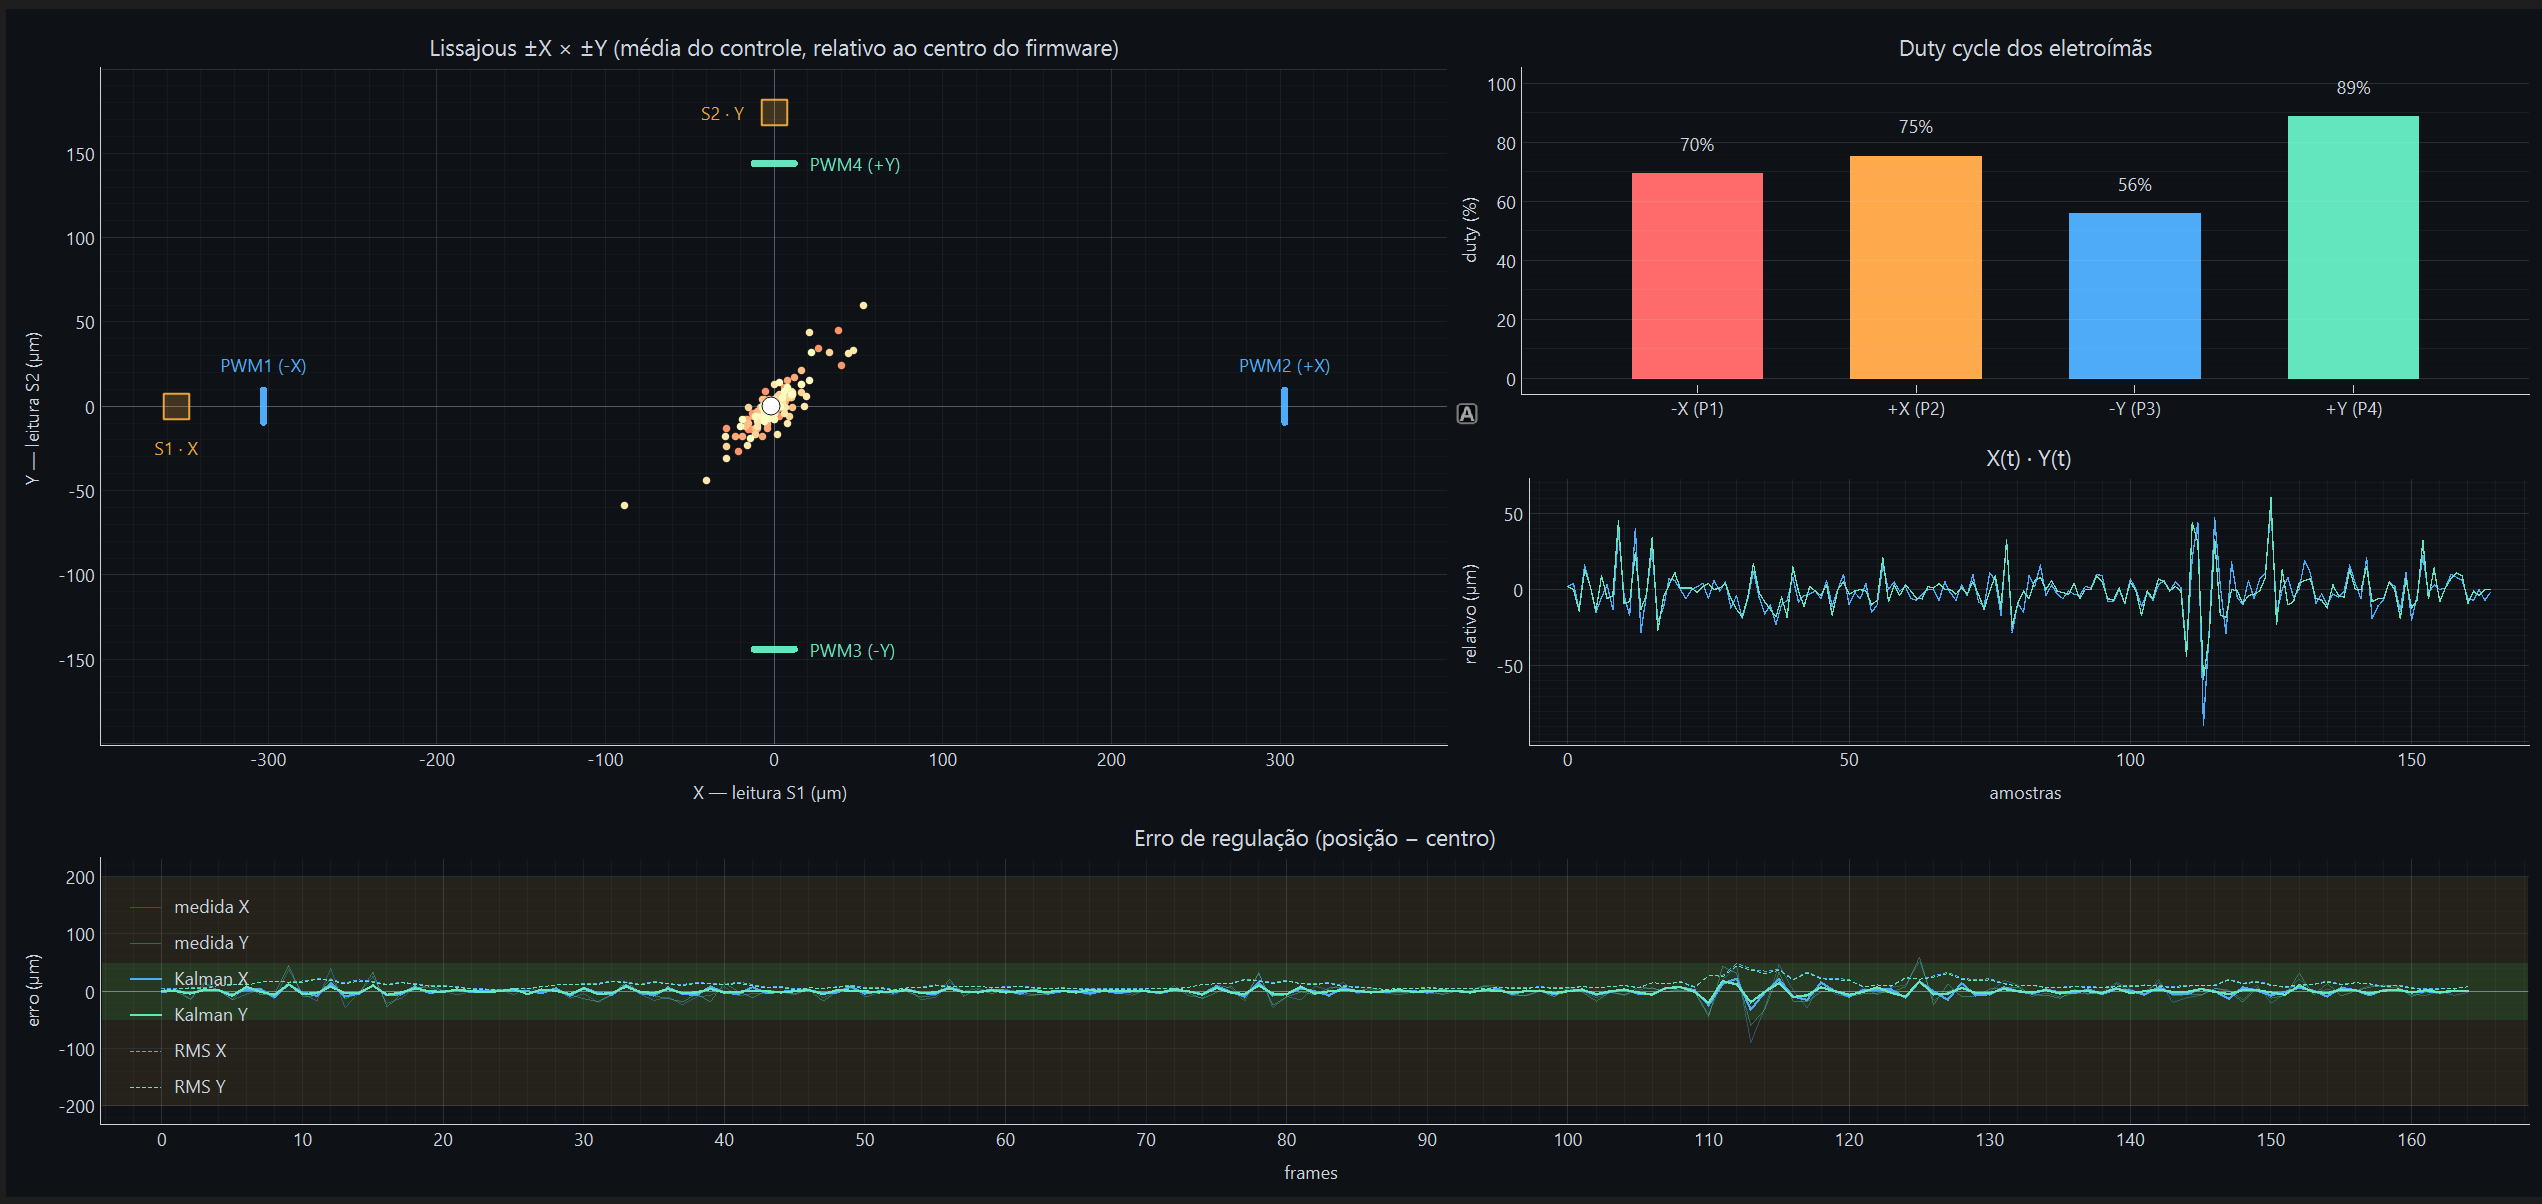
\includegraphics[width=\columnwidth]{supervisor.png}
\caption{Monitoring software on the PC: X and Y position relative to the reference, duty cycles of the four H-bridges, recent positions, and regulation error with the estimator output.}
\label{fig:monitor}
\end{figure}

\section{Experimental Results}\label{sec:results}

\subsection{Procedure}

With the loop closed and the rotor centered, the operator recorded 300 s of telemetry for each blower level (1, 2 and 3) while reading the peak speed on a handheld tachometer (Minipa MDT-2238B). In all three recordings, every frame shows the loop closed and the emergency stop released. Fig.~\ref{fig:time} shows that the recordings include the end of the spin-up and, at levels 2 and 3, the spin-down of the rotor. The analysis therefore uses the window from 30 to 210 s of each recording, shaded in Fig.~\ref{fig:time}, and combines the firmware windows weighted by their cycle count $n$.

\begin{figure}[tbp]
\centering
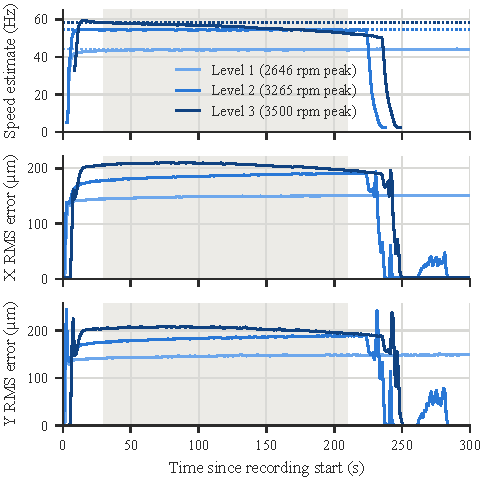
\includegraphics[width=\columnwidth]{time_history.pdf}
\caption{Embedded speed estimate and RMS position error over each recording, in intervals of 1 s. Dotted lines: tachometer peaks. Shaded: analysis window.}
\label{fig:time}
\end{figure}

% Gerado por analysis/extract_results.py; não editar à mão.
% Janela de análise: 30 a 210 s de cada gravação.
\begin{table}[htbp]
\caption{Closed-loop results per blower level, 30 to 210 s of each recording}
\label{tab:results}
\centering
\setlength{\tabcolsep}{4pt}
\begin{tabular}{lccc}
\hline
\textbf{Metric} & \textbf{Level 1} & \textbf{Level 2} & \textbf{Level 3} \\
\hline
Tachometer peak (rpm) & 2646 & 3265 & 3500 \\
Speed est., 99th pct.\ of record (rpm) & 2646 & 3276 & 3558 \\
Speed est., median in window (rpm) & 2622 & 3258 & 3378 \\
RMS error, X/Y ($\mu$m) & $148$/$146$ & $186$/$184$ & $206$/$204$ \\
Peak error, X/Y ($\mu$m) & $334$/$426$ & $395$/$520$ & $423$/$552$ \\
Synchronous amplitude, X/Y ($\mu$m) & $180$/$173$ & $238$/$233$ & $260$/$254$ \\
Mean current, X/Y (mA) & $-14$/$52$ & $-24$/$53$ & $-25$/$51$ \\
Saturated cycles, X/Y (\%) & $0.4$/$7.8$ & $0.0$/$9.8$ & $0.4$/$10.0$ \\
\hline
\end{tabular}
\end{table}


\subsection{Loop Integrity and Speed}

Within the analysis windows, the loop executed between 9999 and 10001 cycles per second of PC time, so no control window was lost, and over the whole recordings it reported no loop errors. Telemetry frames arrived at 16.3 to 16.8 Hz.

The embedded speed estimate agrees with the tachometer (Table~\ref{tab:results}). The tachometer reads a peak, so the comparable estimate is the 99th percentile over each recording: 2646, 3276 and 3558 rpm against tachometer peaks of 2646, 3265 and 3500 rpm, a difference below 1.7 percent. At levels 1 and 2 the speed was steady, between 43.4 and 43.9 Hz and between 54.1 and 54.5 Hz (5th to 95th percentile), and the estimator stayed locked throughout the window. At level 3, unlike levels 1 and 2, the speed drifted down within the window, from 58.1 Hz in its first 10 s to 52.8 Hz in its last 10 s, well before the final spin-down. It stayed above the 55 Hz locking limit for most of the window, and the estimator was locked in only 29 percent of it.

\subsection{Position Error and Control Effort}

\begin{figure}[tbp]
\centering
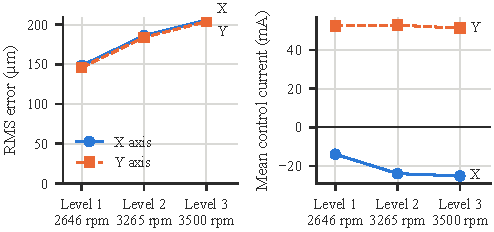
\includegraphics[width=\columnwidth]{summary_levels.pdf}
\caption{RMS position error and mean control current per blower level, from 30 to 210 s of each recording.}
\label{fig:summary}
\end{figure}

The mean position error stayed within 10 $\mu$m of the reference on both axes, as expected from the integral action. The RMS error grew with the blower level, from 148 and 146 $\mu$m (X and Y) at level 1 to 206 and 204 $\mu$m at level 3 (Fig.~\ref{fig:summary}). Most of it occurs at the rotation frequency: the synchronous amplitude reported by the speed estimator accounts for 70 to 84 percent of the error variance on the locked frames. Since the probes read a target ring, this component includes the runout of the ring as well as the motion of the rotor. The largest peak error, 552 $\mu$m on Y at level 3, remained below half of the 1.45 mm nominal gap.

The two axes differ in effort. The X axis drew a mean control current between $-25$ and $-14$ mA and saturated in at most 0.4 percent of the cycles. The Y axis drew a nearly constant $+51$ to $+53$ mA, more than a third of the 140 mA control range, and saturated in 7.8 to 10.0 percent of the cycles. The integral action thus holds a static load on Y and leaves less range for the synchronous demand. Earlier bench sessions showed the same behavior with the rotor at rest and with other position references, with 46 to 59 mA on Y. Since both axes are radial and the weight rests on the pivot, this load is not gravity; it points to an asymmetry between the two Y electromagnets or their driver channels.

\section{Discussion: Model Versus Bench}\label{sec:discussion}

The design model and the bench disagree in several respects. The differences are expected, since the model was built to stabilize a rotor at rest, and each one points to a missing element of the model or of the instrumentation.

\emph{Error level.} At rest the model and the bench agree: the simulation predicts a standard deviation of about 2 $\mu$m at the probe, and earlier bench sessions measured 2.1 to 3.6 $\mu$m of noise after the notch. While spinning, the bench shows 146 to 206 $\mu$m RMS. The design model has no rotation-dependent excitation: it contains neither mass unbalance, whose force grows with the square of the speed, nor the runout of the target ring. With the ring secured, turning the rotor by hand with the coils off still traced a runout circle of about 146 $\mu$m radius at the probe, a reading that the controller treats as displacement and answers with synchronous current. Both effects act at the rotation frequency, where 70 to 84 percent of the measured variance lies. Centering the ring, modeling the unbalance, and rejecting the remainder with synchronous compensation~\cite{zhao2026constraint}, disabled in these tests, are the corresponding steps.

\emph{Static load.} The design assumed a constant disturbance of 40 mA per axis and the same PMB on both axes. The bench needed 14 to 25 mA on X, inside that assumption, but about 52 mA on Y, consistent with the asymmetry noted in Section~\ref{sec:results}. The integral action absorbed it at the cost of control range: Y saturated in 7.8 to 10.0 percent of the cycles where the simulation predicted none. Balancing the Y channels, or designing with the measured load, is the corresponding step.

\emph{Second mode.} The regulator leaves the second mode pair of the model at 65 Hz with a damping ratio of 0.017, and the speed reached about 59 Hz at level 3. Closed-loop identification on development builds placed this mode near 77 to 80 Hz, which suggests a stiffer shaft than modeled, and revealed an actuator lag of about 2 ms, consistent with the coil time constant that the model omits. The growth of the error with speed is consistent both with an unbalance force that rises with the square of the speed and with the approach to this lightly damped mode, and the window statistics cannot separate the two. A design on the identified plant, with a weight on the modal velocity of the second pair, would address it.

\emph{Stability margin.} The worst case of the grid kept a small margin, a pole at $-1.1$ s$^{-1}$, when the PMB damping is lowest. The bench did not lose stability in any recording, but its margin was not measured. Measuring the sensitivity function, as ISO 14839-3 prescribes for AMB machinery~\cite{iso14839_3}, would quantify it.

\emph{Speed estimator.} The embedded estimator matched the tachometer, but its locking range ends at 55 Hz, which the rotor exceeded at level 3. Widening that range is necessary before the estimator drives any synchronous compensation.

\section{Limitations}\label{sec:limitations}

The results carry the following limitations.
\begin{itemize}
\item \emph{Speed.} The rotation speed was not recorded synchronously with the telemetry, and the recording labels are not speed measurements. The only speed data are the embedded estimate and the peak read on a handheld tachometer.
\item \emph{Timing.} Each recording starts when the operator requests it, and its time stamps are PC reception times, not controller time. The analysis window is defined on this time base.
\item \emph{Sampling.} At 16.3 to 16.8 Hz, the telemetry is slower than the control loop and slower than the rotation (43 to 59 Hz), so single samples alias the rotating orbit. For this reason, the analysis uses only the window statistics and draws no orbit from the samples.
\item \emph{Statistics.} The cycle count $n$, mean, RMS, peak and saturation are firmware window statistics, truncated to integer micrometers and microamperes before transmission.
\item \emph{Actuator.} Without current sensing, the coil currents follow \eqref{eq:duty} only in steady state.
\item \emph{Model.} The controller was designed on the nominal model, with PMB stiffness and damping assumed rather than identified, and the same parameters for both axes.
\item \emph{Reference, runout and execution time.} The position reference approximates the bearing center, the measured error includes the runout of the target ring, and the execution time of the control step was measured only on development builds, not on the tested one.
\item \emph{Operating point.} At level 3 the speed was not stationary within the analysis window.
\end{itemize}

\section{Conclusion}\label{sec:conclusion}

A ten-state LQG controller with integral action, derived from an FE rotor model through modal truncation, a sensor-referenced state, discrete design and a robustness grid, ran at 10 kHz on a TMS320F28379D and kept a vertical rotor centered up to about 3500 rpm on a bench without current sensing. Over three recordings of 300 s the loop kept its rate without errors, and the embedded speed estimator matched the tachometer within 1.7 percent. The error is dominated by the synchronous component, and the Y axis spends up to 10 percent of the cycles in saturation while it holds a static load. Where the bench departed from the design model, the departures point to the next iteration: design on the plant identified per axis, center the target ring, balance the Y channels, add damping to the second mode pair, measure the stability margin and the execution time on the tested build, and enable synchronous compensation, as in~\cite{zhao2026constraint}, before the controller moves to the full-scale FESS.

\section*{Acknowledgment}

% Declaração de uso de IA exigida pela IEEE (CLAUDE.md, seção 8.3). O autor deve confirmar.
The authors used Claude Opus 5.5 (Anthropic), a large language model, to write the data analysis script that produced Figs.~\ref{fig:time} and~\ref{fig:summary} and Table~\ref{tab:results}. The authors reviewed the script and its outputs and take full responsibility for them.

\bibliographystyle{IEEEtran}
\bibliography{IEEEabrv,refs}

\end{document}
